\documentclass[addpoints,spanish, 12pt,a4paper,cancelspace]{./include/gexam}

 %%%%%%%%%%%%%%%%%%%%%%%%%%%
 \renewcommand{\documentName} { 3ª evaluación }
 \renewcommand{\documentContent} { Sistema de coordenadas cartesianos } 
 \renewcommand{\waterMark} { Modelo B } 

 % Configuración del documento.
 \renewcommand{\schoolSubject} { Examen Matemáticas 2º ESO  }
\renewcommand{\school} { IES José de Churriguera  }
\renewcommand{\academicPeriod} { Curso 2022/2023 }

\renewcommand{\autor} { Andrés Giménez Muñoz }
\renewcommand{\emailAuthor} { andresprofemates@outlook.es }
\renewcommand{\autorSing}{ Profesor: Andrés } 
 %%%%%%%%%%%%%%%%%%%%%%%%%%%
 
% \renewcommand{\thepartno}{\arabic{partno}}
%  \renewcommand{\thepartno}{\thecurrentpartno.\arabic{partno}}

% \renewcommand{\partlabel}{(\thequestion.\arabic{partno})}
% \renewcommand{\subpartlabel}{(\thepart.\arabic{subpartno})}

\renewcommand\subpartlabel{(\thesubpart)}
\renewcommand\subpartshook{\renewcommand\makelabel[1]{##1\hfil }} 
 
 %%%%%%%%%%%%%%%%%%%%%%%%%%%
 % Exam configuration
 %\pointsdroppedatright   %% No mostrar la puntuación
 \pointsinrightmargin{} % Para poner las puntuaciones a la derecha. Se puede cambiar. Si se comenta, sale a la izquierda.
 \extrawidth{-1.5cm} %Un poquito más de margen por si ponemos textos largos.
 \marginpointname{ \emph{\points}}
 
 %% Si se comenta no aparecerán los espacios de la solución.
 %\nocancelspace
 
 %% Puntuación a la izquierda.
%  \nopointsinrightmargin 

 %% Esto es de la clase exam. Si dejamos sin comentar \printanswers, se mostraran las soluciones. 
 %% Si la comentamos y dejamos sin comentar \noprintanswers, pues no se muestran las soluciones.
 % \printanswers
 %\noprintanswers
 
 %%%%%%%%%%%%%%%%%%%%%%%%%%%
 
 \begin{document}
 
 \StudentData{}
 \GradeTableHeader{}
 
 \justifying{}

 \justifying

% \begin{center}
%     \fbox{\fbox{\parbox{6.5in}{             
%                 \begin{itemize}
%                     \item Deben aparecer todas las operaciones, no vale solo con indicar el resultado.
%                     \item Se podrán quitar hasta cinco décimas por falta de claridad o rigor en el desarrollo de las respuestas o por una mala presentación.
%                     \item Se valorará que se indiquen las cuentas en línea, realizando las operaciones en el margen.
%                     \item No se puede utilizar la calculadora.
%                 \end{itemize}
%             }}}
% \end{center}
 
 \begin{questions}
    
    %% Buo
    \question[1] Dibuja los puntos en el orden en el que aparece y únelos con segmentos de línea. \\
    Trazo 1:
    \\
    $(4, 3)$, $(5, 7)$, $(6, 10)$, $(8, 14)$, $(7, 16)$, $(6, 19)$, $(6, 21)$, $(7, 23)$, $(8, 24)$, $(9, 25)$, $(8, 28)$, $(8, 30)$, 
    $(12, 27)$, $(26, 27)$, $(30, 30)$, $(30, 28)$, $(29, 25)$, $(31, 22)$, $(32, 20)$$(32, 18)$, $(31, 15)$, $(30, 14)$, $(32, 10)$, 
    $(34, 5)$, $(35, 0)$, $(36, -10)$, $(36, -15)$, $(35, -20)$, $(34, -25)$, $(32, -33)$, $(36, -32)$$(39, -30)$, $(44, -27)$, 
    $(48, -25)$, $(47, -28)$$(45, -31)$, $(42, -34)$, $(38, -38)$, $(35, -40)$$(32, -42)$, $(27, -44)$, $(25, -51)$,
    $(23, -51)$$(21, -53)$, $(19, -53)$, $(18, -55)$, $(13, -55)$, $(7, -48)$, $(2, -48)$, $(-5, -46)$, $(-14, -42)$, 
    $(-20, -38)$, $(-24, -35)$, $(-28, -30)$, $(-32, -25)$, $(-35, -20)$, $(-37, -15)$, $(-38, -10)$, 
    $(-39, -5)$, $(-40, 0)$, $(-40, 5)$, $(-39, 12)$$(-38, 18)$, $(-36, 25)$, $(-33, 30)$, $(-30, 35)$, $(-24, 40)$, 
    $(-20, 43)$, $(-15, 46)$, $(-10, 48)$, $(-5, 50)$, $(-1, 51)$, $(5, 52)$, $(20, 52)$, $(30, 51)$, $(34, 49)$, 
    $(25, 49)$, $(15, 48)$, $(10, 47)$, $(3, 45)$, $(-1, 43)$, $(-5, 40)$, $(-5, 40)$, $(-11, 35)$, $(-15, 30)$, $(-18, 24)$,
    $(-20, 18)$, $(-21, 13)$, $(-21, 5)$, $(-20, -4)$, $(-18, -10)$, $(-16, -15)$, $(-10, -23)$, $(-5, -28)$, $(0, -31)$,
    $(4, -33)$, $(3, -30)$, $(2, -20)$, $(2, -15)$, $(2, -5)$, $(4, 3)$
    \\
    Trazo 2:
    \\
    $(14, 22)$, $(14, 20)$, $(17, 20)$
    \\
    Trazo 2:
    \\
    $(21, 20)$, $(24, 20)$, $(24, 22)$
    \\

    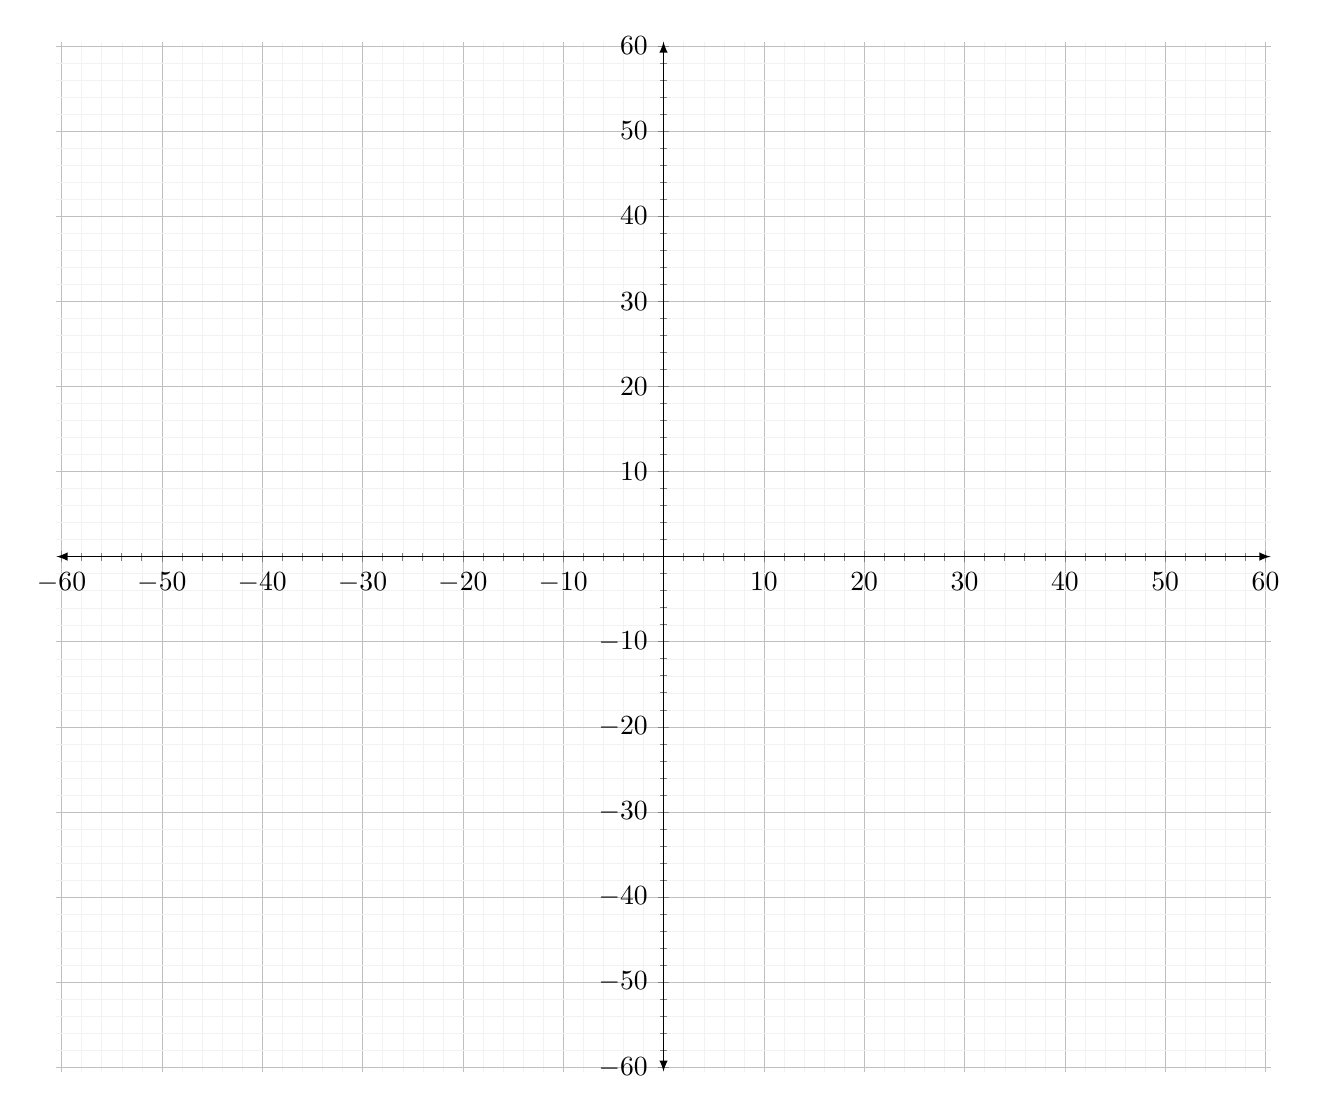
\begin{tikzpicture}[scale=1]
        \begin{axis}[
            axis x line=center,
            axis y line=center,
            xmin=-60,xmax=60,
            ymin=-60,ymax=60,
            grid=both,
            grid style={line width=.1pt, draw=gray!10},
            major grid style={line width=.2pt,draw=gray!50},
            axis lines=middle,
            axis line style={<->},
            minor tick num=4,
            enlargelimits={abs=0.5},
            axis line style={latex-latex},
            % ticklabel style={font=\tiny,fill=white},
            % xlabel style={at={(ticklabel* cs:1)},anchor=north west},
            % ylabel style={at={(ticklabel* cs:1)},anchor=south west},
            xlabel style={below right},
            ylabel style={above left},
            width=17cm,
        ]
        
        \end{axis}

    \end{tikzpicture}

\end{questions}
 
\end{document}